% !TEX encoding = UTF-8 Unicode
% !TEX root = thesis-ex.tex


This discussion is based on Ref.~\cite{PhysRevLett.88.022301}.
Done at RHIC by the PHENIX collaboration, this was one of the first experimental measurements of jet quenching that showed the presence of the QGP.
This measurement analyzed high \pt\ charged hadrons and neutral $\pi^0$s ($\pt > 2$ GeV) from jets produced in \AuAu\ collisions, collided at $\sqrtsnn = 130$ GeV.
Since jets form early in the collision and experience the evolution of the QGP, they are expected to lose energy due to collisional and radiative losses as discussed in Section~\ref{sec:jets}.
The modifications between the \pp\ and \AuAu\ system was quantified by constructing the nuclear modification factor \RAA, given as:

\begin{align}
\RAA_{\pt} = \frac{(1 / \Nevt) d^2 N^{\rm A+A} / d\pt d\eta}{(\langle N_{\rm binary} \rangle / \sigma_{\rm inel}^{\rm N+N} d^2 \sigma^{\rm N+N} / d\pt d\eta}
\end{align}
where \Nevt\ is the number of \AuAu\ events, $\langle N_{\rm binary} \rangle$ is the average number of binary collisions per event, $\sigma$ is the scattering cross section, and \pt\ and $\eta$ are the kinematics of the charged particle.

The \RAA\ for charged hadrons and neutral pions is shown in Figure~\ref{fig:hadron_raa}.
A significant depletion is seen, with the \RAA\ rising for $\pt < 2$ GeV and remaining fairly constant thereafter.
Electroweak probes like photons and Z bosons do not lose energy is the QGP since they do not interact strongly, and their \RAA\ is expected to be closer to unity.
This can be seen in Figure~\ref{fig:photon_raa}
Some other \RAA\ measurements from RHIC and the LHC include \cite{PhysRevLett.91.172302, PhysRevLett.91.072301, PhysRevC.70.061901, 201130, Chatrchyan2012, Khachatryan:2016odn, ATLAS-CONF-2017-012}.

\begin{figure}
\begin{subfigure}{.5\textwidth}
\centering
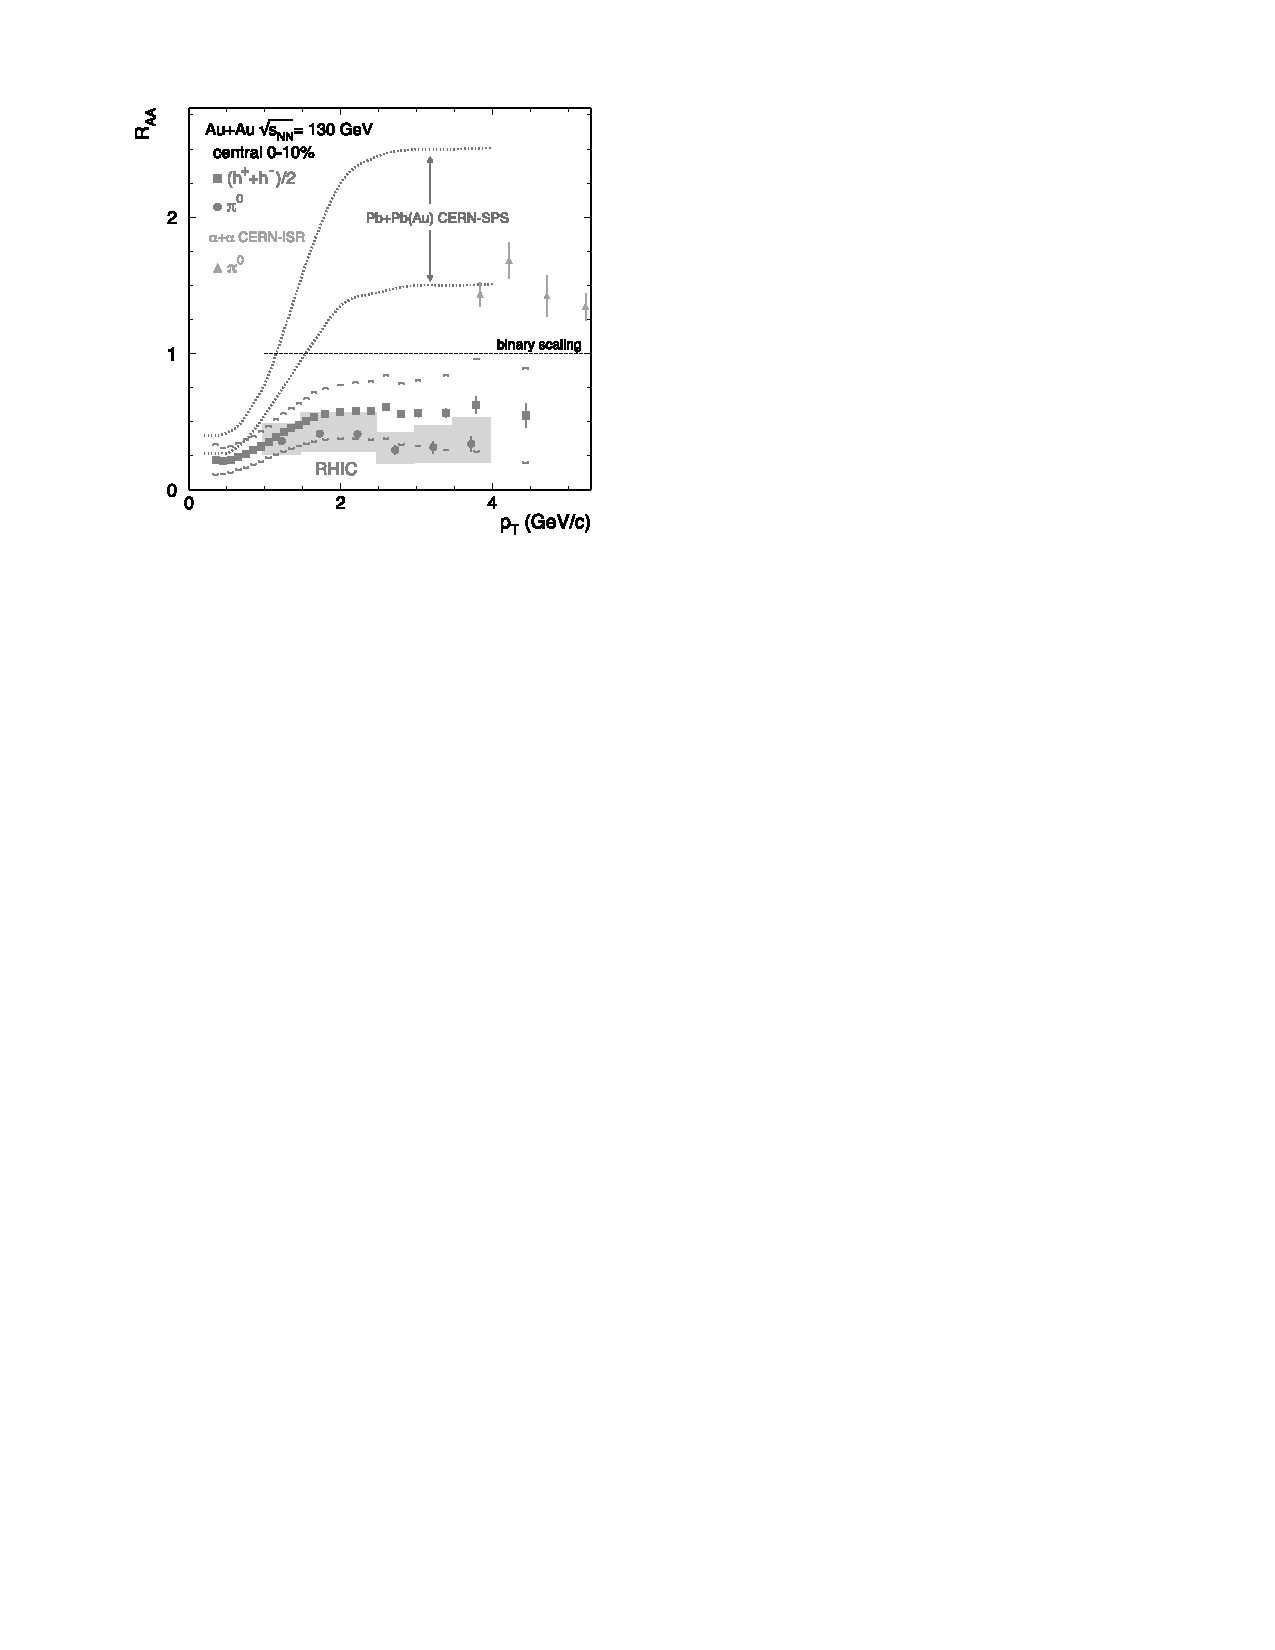
\includegraphics[width=\textwidth]{figures/jetMeasurements/hadron_raa}
\caption{The \RAA\ for charged hadrons and neutral pions in \AuAu\ collisions at $\sqrtsnn = 130$ GeV.
Also shown is the \RAA\ for inclusive cross sections in $\alpha+\alpha$ compared to \pp\ at $\sqrtsnn = 31$ GeV \cite{ANGELIS1987213} and spectra from \pbpb and $\rm{Pb}+{\rm AU}$ compared to \pp\ at $\sqrtsnn = 17$ GeV \cite{PhysRevC.64.034901}.
Figure from Ref.~\cite{PhysRevLett.88.022301}.}
\label{fig:hadron_raa}
\end{subfigure} \qquad
\begin{subfigure}{.5\textwidth}
\centering
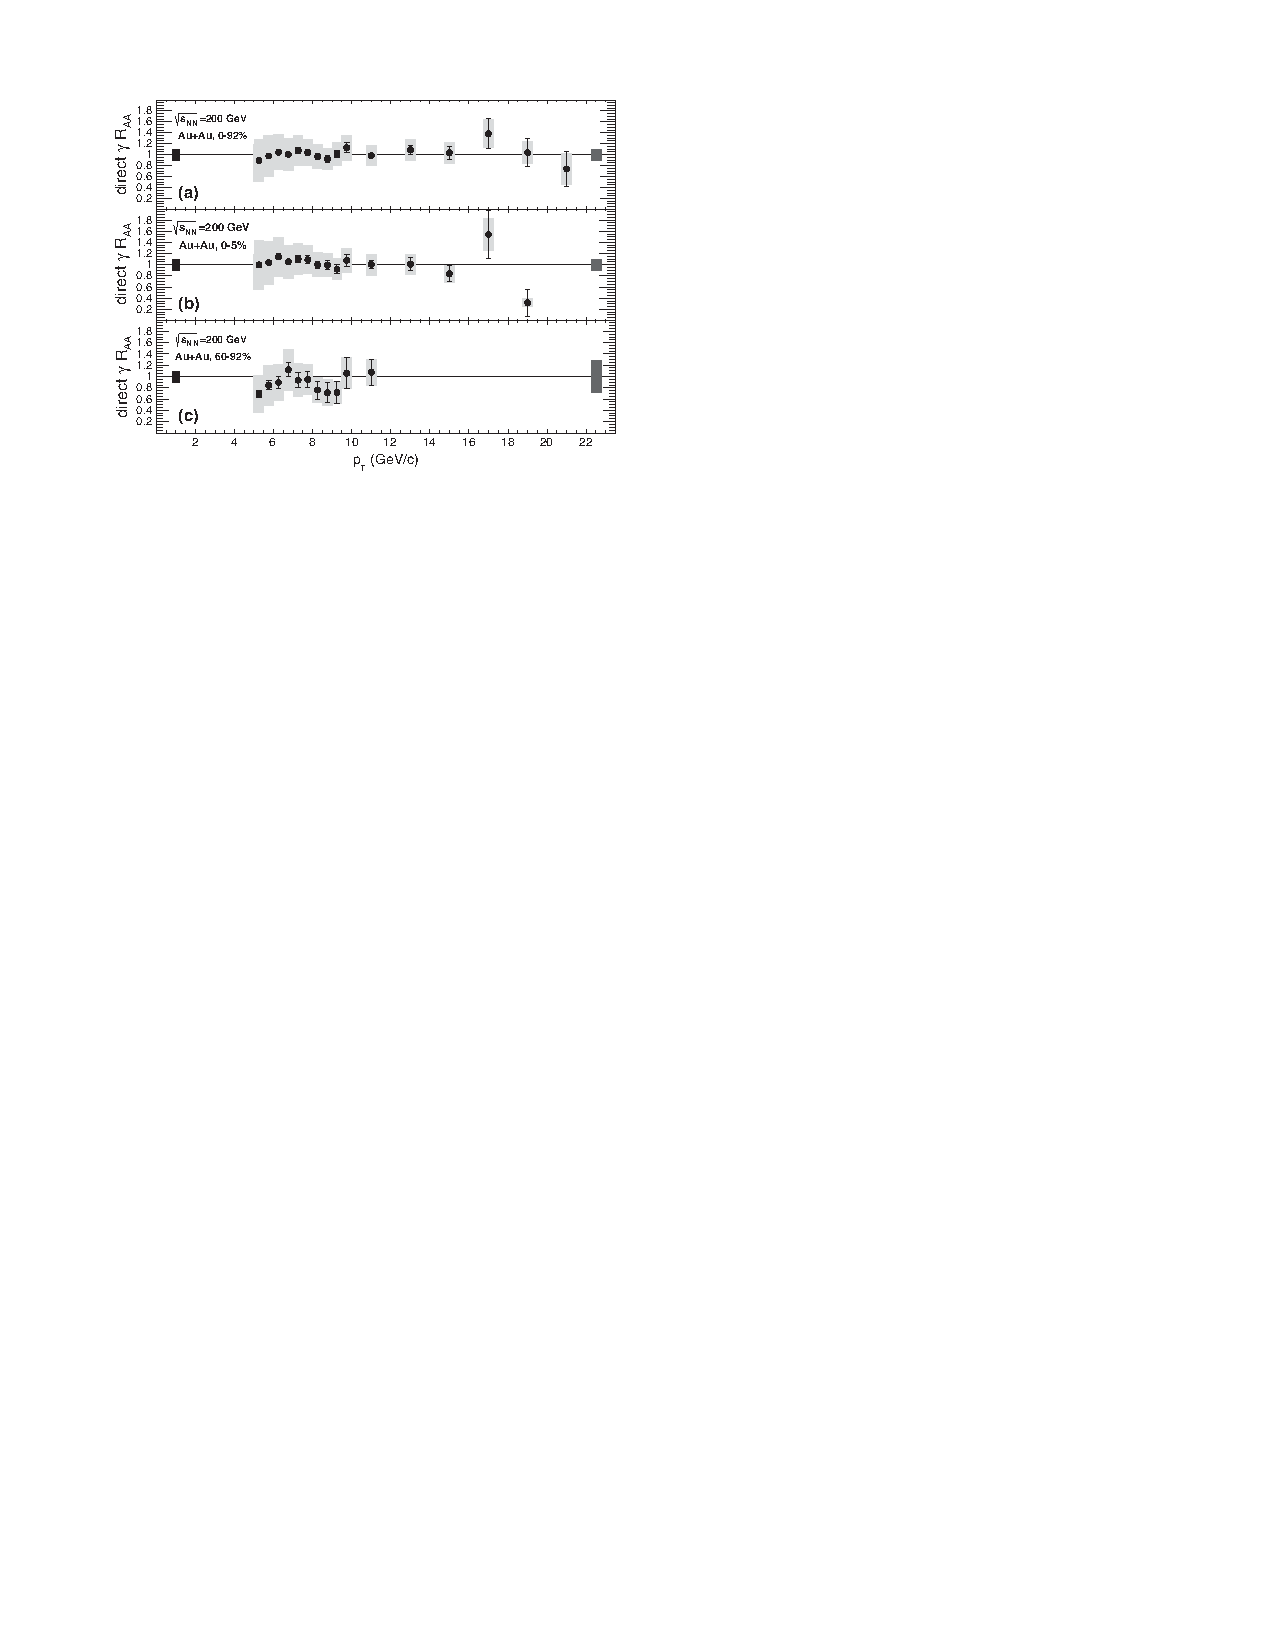
\includegraphics[width=\textwidth]{figures/jetMeasurements/photon_raa}
\caption{The \RAA\ for photons as a function of \pt\ for three centrality selections in \AuAu\ collisions at $\sqrtsnn = 200$ GeV.
Figure from Ref.~\cite{PhysRevLett.109.152302}.}
\label{fig:photon_raa}
\end{subfigure}
\caption{\RAA\ evaluated for (left) charged hadrons and pions and (right) photons.}
\label{fig:particle_raa}
\end{figure}


